
%\font\bfbig=cmbx10 scaled\magstep4  
%\font\bftitle=cmbx10 scaled\magstep1
%\font\smbftit=cmbx10 scaled\magstep2
%\font\amb=cmtt10 scaled\magstep0
%\font\bgtt=cmtt10 scaled\magstep1

% The "twoside" in documentstyle sets positioning of 
% page numbers on the page./
%   \documentstyle[fullpage,twoside]{report}
\documentclass[a4paper]{article}
\addtolength{\hoffset}{-15mm}
\addtolength{\textwidth}{3cm}
\addtolength{\textheight}{3.5cm}
\usepackage{makeidx,graphicx}
\usepackage{fix-cm}
\makeindex
%\newcommand{\HRule}{\rule{\linewidth}{0.5mm}}

\begin{document}


% \begin{titlepage}

% \begin{center}

% % Upper part of the page
% \vspace*{2.0in}
% % \begin{figure}[h!]
% 
\includegraphics[width=1\textwidth]{./Hawk2.png}\\[1cm] 
% \label{hawk-cover}   
% % \end{figure}

% { \Huge \textsc{Quickstart Guide}}\\[1.4cm]

% %\vspace{0.3in}
% % Author and supervisor
% \begin{minipage}{0.2\textwidth}
% \begin{flushleft} \large
% Filipe Maia
% \end{flushleft}
% \end{minipage}
% \begin{minipage}{0.2\textwidth}
% \begin{flushright} \large
% Tomas Ekeberg
% \end{flushright}
% \end{minipage}

% \vfill

% % Bottom of the page
% {\large \today}

% \end{center}

% \end{titlepage}

\title{
\vspace*{-1in}
\begin{figure}[!h]
%\centering

\includegraphics[width=15cm]{Hawk2.png}
\label{hawk-cover}
\end{figure}
\vspace {0.5in}
{\fontsize{30}{40}\fontfamily{ptm}\selectfont \textbf{Quickstart Guide} }}
\author {\huge Filipe Maia}


\maketitle

\parindent=0pt 
\baselineskip=18pt 
\lineskip=0pt
\pagenumbering{roman}

%\tableofcontents

\pagestyle{headings}

\def\delfo{$\delta_{fo}$~}
\def\delfc{$\delta_{fc}$~}
\def\qq{\qquad\qquad}
\def\hbar{\overline{h}}


% OFF WE GO .......

\section{Introduction} 
\label{intro}
\pagenumbering{arabic}

\vspace {0.1in}

This is a small document with the objective of introducing you to the
diffraction imaging reconstruction software Hawk.
Hawk is a collection of computer programs which aim at reconstructing an object from 
it's oversampled  diffraction pattern.


\section{Opening the Experimental Data}
\label{tutorial}

Hawk supports both its own hdf5 data files and tiff files.
If you have another kind of file probably the easiest is to try to
convert it to a tiff file.

In this guide we will reconstruct a simple object, a ring. I'm going
to assume you have Hawk installed and all the programs are in the path. If
this is not the case please read the User Manual for further
instructions.

Inside the Hawk directory there should be a file called
``examples/ring/raw\_ring.h5.gz''. Extract that file using gunzip.
This file contains the experimental diffraction intensities recorded
using a laser pointer shinning on a small ring.

Now start the HawkGUI, and select the Editor Tab (Fig. \ref{select-editor}).

\begin{figure}[h]
 \centering
 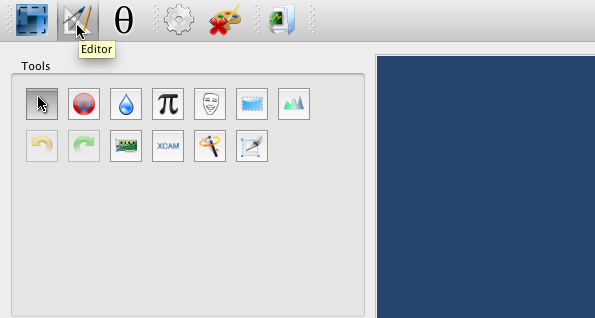
\includegraphics[width=0.6\textwidth]{./select_editor.png}
\caption{The top left three icons define the three workspace in
   Hawk. We are selecting the editor to take an initial look at the
   experimental data.}
 \label{select-editor}   
\end{figure}

Now load the file from disk by clicking on the folder icon (Fig. \ref{load-file}).

\begin{figure}[h!]
\centering
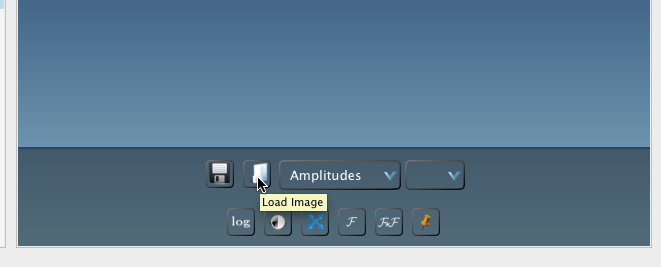
\includegraphics[width=0.8\textwidth]{./load-file.png}
\caption{Loading a file from the popup toolbar on the bottom of the
  editor working area.}
\label{load-file}   
\end{figure}

If everything went according to plan you should now see the
experimental data (Fig. \ref{raw-ring}).

\begin{figure}[h!]
\centering
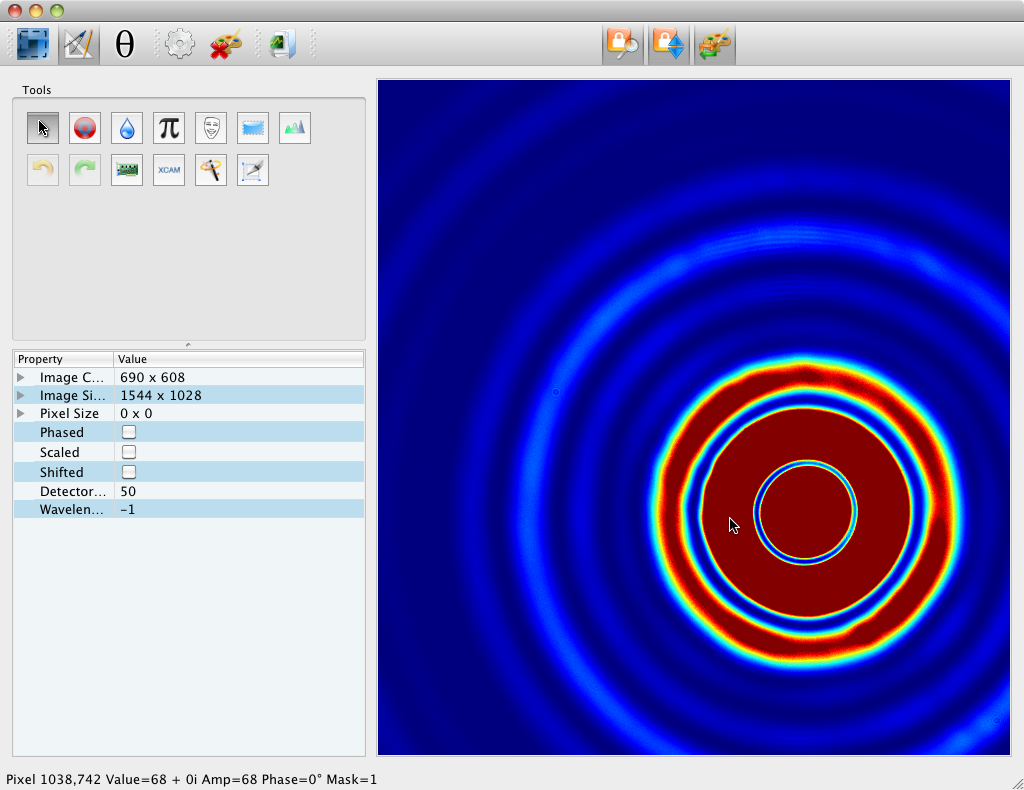
\includegraphics[width=0.8\textwidth]{./raw-ring.png}
\caption{Screenshot just after loading ``raw\_ring.h5'' into the
 editor. You can zoom in and out by pressing the right mouse button
 and dragging, and pan using the left mouse button.}
\label{raw-ring}   
\end{figure}


\section{Defining Masks}

Notice that many parts of the image are bright red. This is usually a
sign that the detector saturated in those regions, and so the
value there is not the correct measurement of the received intensity.
We'll have to indicate to the program that we do not have information
about these saturated regions.

We'll do this by removing those pixels from the mask of valid values.
First to be able to see the current mask go to popup image menu and
select ``Shaded Mask'' (Fig. \ref{select-shaded-mask.png}).
There should be no change as everything is part of the mask.

\begin{figure}[h!]
\centering
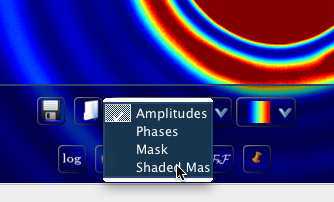
\includegraphics[width=0.5\textwidth]{./select-shaded-mask.png}
\caption{Making the mask visible by changing the current display mode.}
\label{select-shaded-mask}   
\end{figure}

Now click on the ``Edit image mask'' tool and the select the mode
``Exclude from mask''. Your mouse should now have turned into a small
circle, when it's overing over the work canvas, and you should be able
to click on the image to exlude those pixels from the mask. They will
subsequently turn darker, indicating that they have been excluded from
the mask (Fig. \ref{exclude-from-mask}). Try to mask out all the
bright red pixels. You can change the size of the brush to make the
work go faster. This is usually a tedious, but essential, task.

\begin{figure}[h!]
\centering
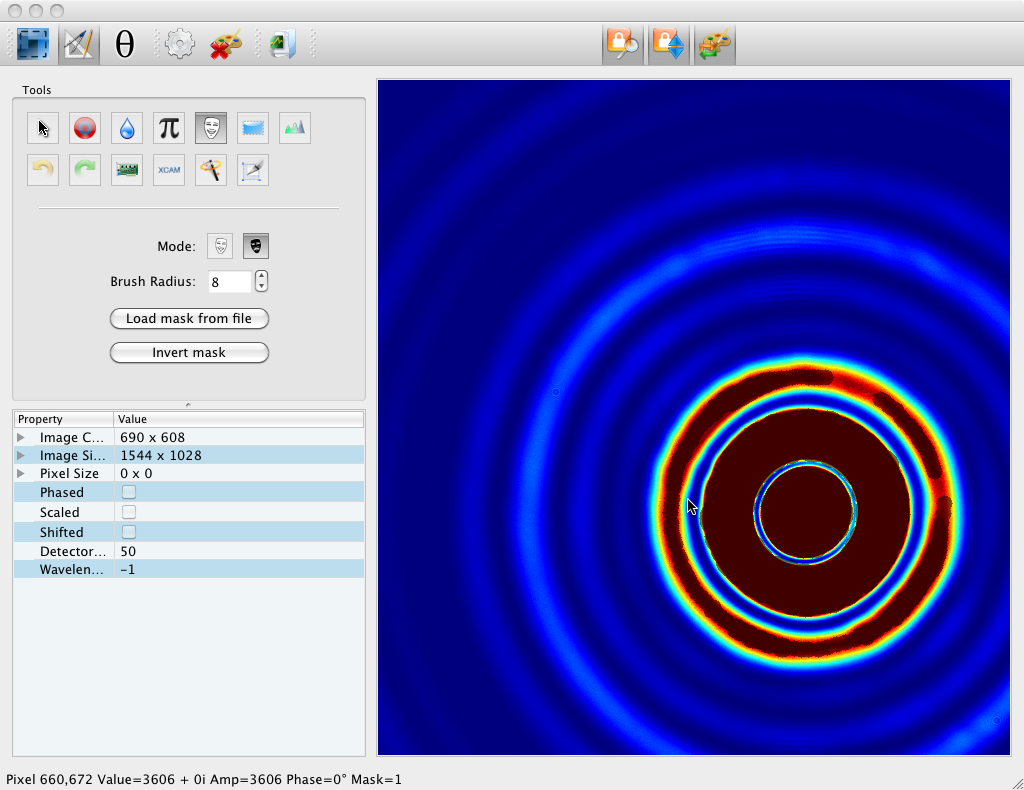
\includegraphics[width=0.9\textwidth]{./after-masking.png}
\caption{Raw ring after masking.}
\label{select-shaded-mask}   
\end{figure}

Now we'll define the center of the diffraction pattern. This step is
essential when one tries to use reality constraints, as the constraint
is only valid when the center is determined exactly. In our case we'll
not use such constraint, but it's still good practice to set the
center. The tool that defines the image center is called ``Set Image
Center''. Just select it and then click on the desired image center
(Fig. \ref{find-center}).

\begin{figure}[h!]
\centering
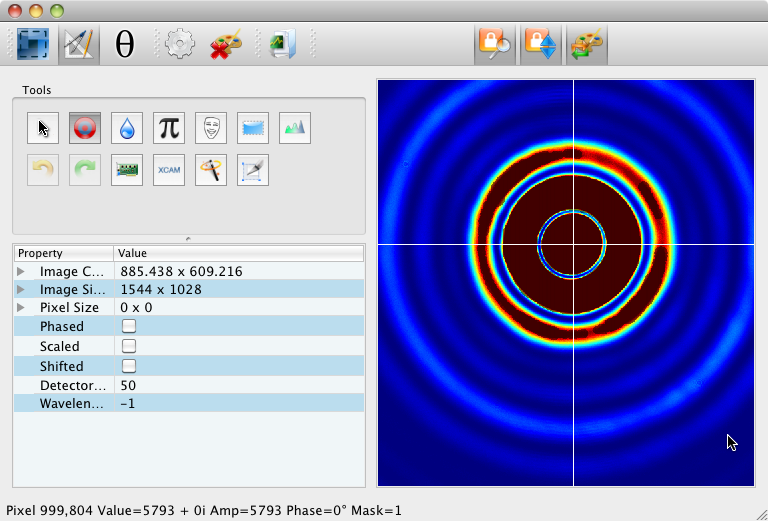
\includegraphics[width=0.8\textwidth]{./find-center.png}
\caption{Raw ring with the center defined.}
\label{find-center}   
\end{figure}

Now that the image is ready to be used, saved it with another
name. I'll use ``ring\_edited.h5''. 

\section{Downsampling the Original Data}

You might have noticed that the ring image was very large and smooth. 
To make calculations faster we can use only a subset of the image, and
in this case still achieve an image as good as if we had used the
entire image. We'll use the command line tool ``process\_image'' for
this. We'll downsample the image 3 times with:

\qq {\tt  \$ process\_image -i ring\_edited.h5 -o ring\_downsampled.h5 -a 3}

If you want you can take a look at the resulting image in the editor.
We'll try to integrate this part in the graphical interface in the
near future.

\section{Reconstructing the Ring}

Now we'll try to reconstruct the image of the ring. To do that first
go to the Phaser workspace (just click on the big $\Theta$).

On the left hand side there are a bunch of options, some of which
we'll have to define. They control the reconstruction. 
By overing the mouse over each of the options, you will see a small
help text which should help you understand what each one does.

The first thing
to define is the ``Input Data''. Set the ``Intensities File'' to the
file that you just saved (``ring\_downsampled.h5'' in my case).

Now open the Phasing Method entry. The ``hio'' Phasing Algorithm
should be selected. If you want you can try other algorithms.

Now take a look at the ``Support Update Method'' entry.
The ``Support Update Algorithm'' should be set to area, which is an
algorithm that lets you constrain the area of the reconstructed
object. The ``Object Area'' is set to 0.001, which means that only
0.1\% of the total image area will be occupied by the reconstructed
object. Click on the ``Object Area'' value and an editor should show
up (Fig. \ref{object-area-editor}). Double click on the left hand side
control point and change the value to 0.01.  This mean that we'll
constrain the area in the beggining of the reconstruction to 1\% of the
total image area. Change the right hand side control point value to
0.003. This means that the after 2000 iterations the object will be
constrained to an area of 0.3\% the total area.

\begin{figure}[h!]
\centering
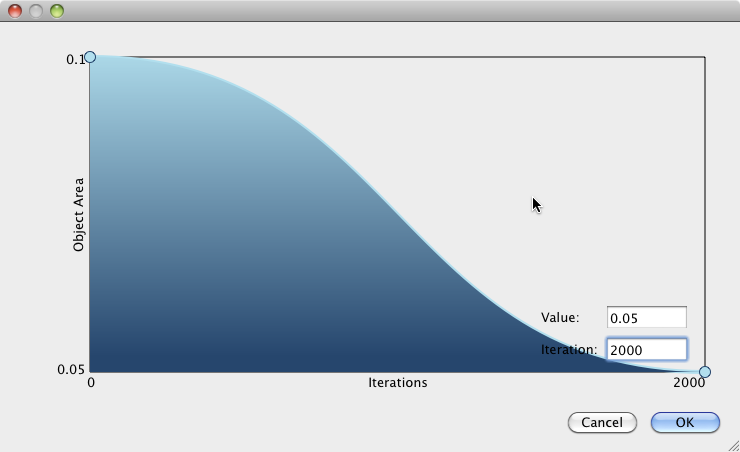
\includegraphics[width=0.8\textwidth]{object-area-editor.png}
\caption{Object Area editor after being adjusted for the ring.}
\label{object-area-editor}   
\end{figure}
 
Finally go to ``Logging'' entry and set the ``Working Directory'' that
you prefer. This is the directory where all the output files will be
written to. You can change the frequency at which statistics are
output to the log file by changing ``Log Output Period'' and the
frequency at which images are saved to disk, by changing ``Images
Output Period''. I created a directory called ``output'' inside the
ring examples directory and set it to the ``Working Directory''.

Now hit the ``Run'' button, and after some seconds you should see some action.
If everything went well, after a couple thousands iterations you
should see a distorted ring emerge (Fig. \ref{reconstructed-ring}).

\begin{figure}[h!]
\centering
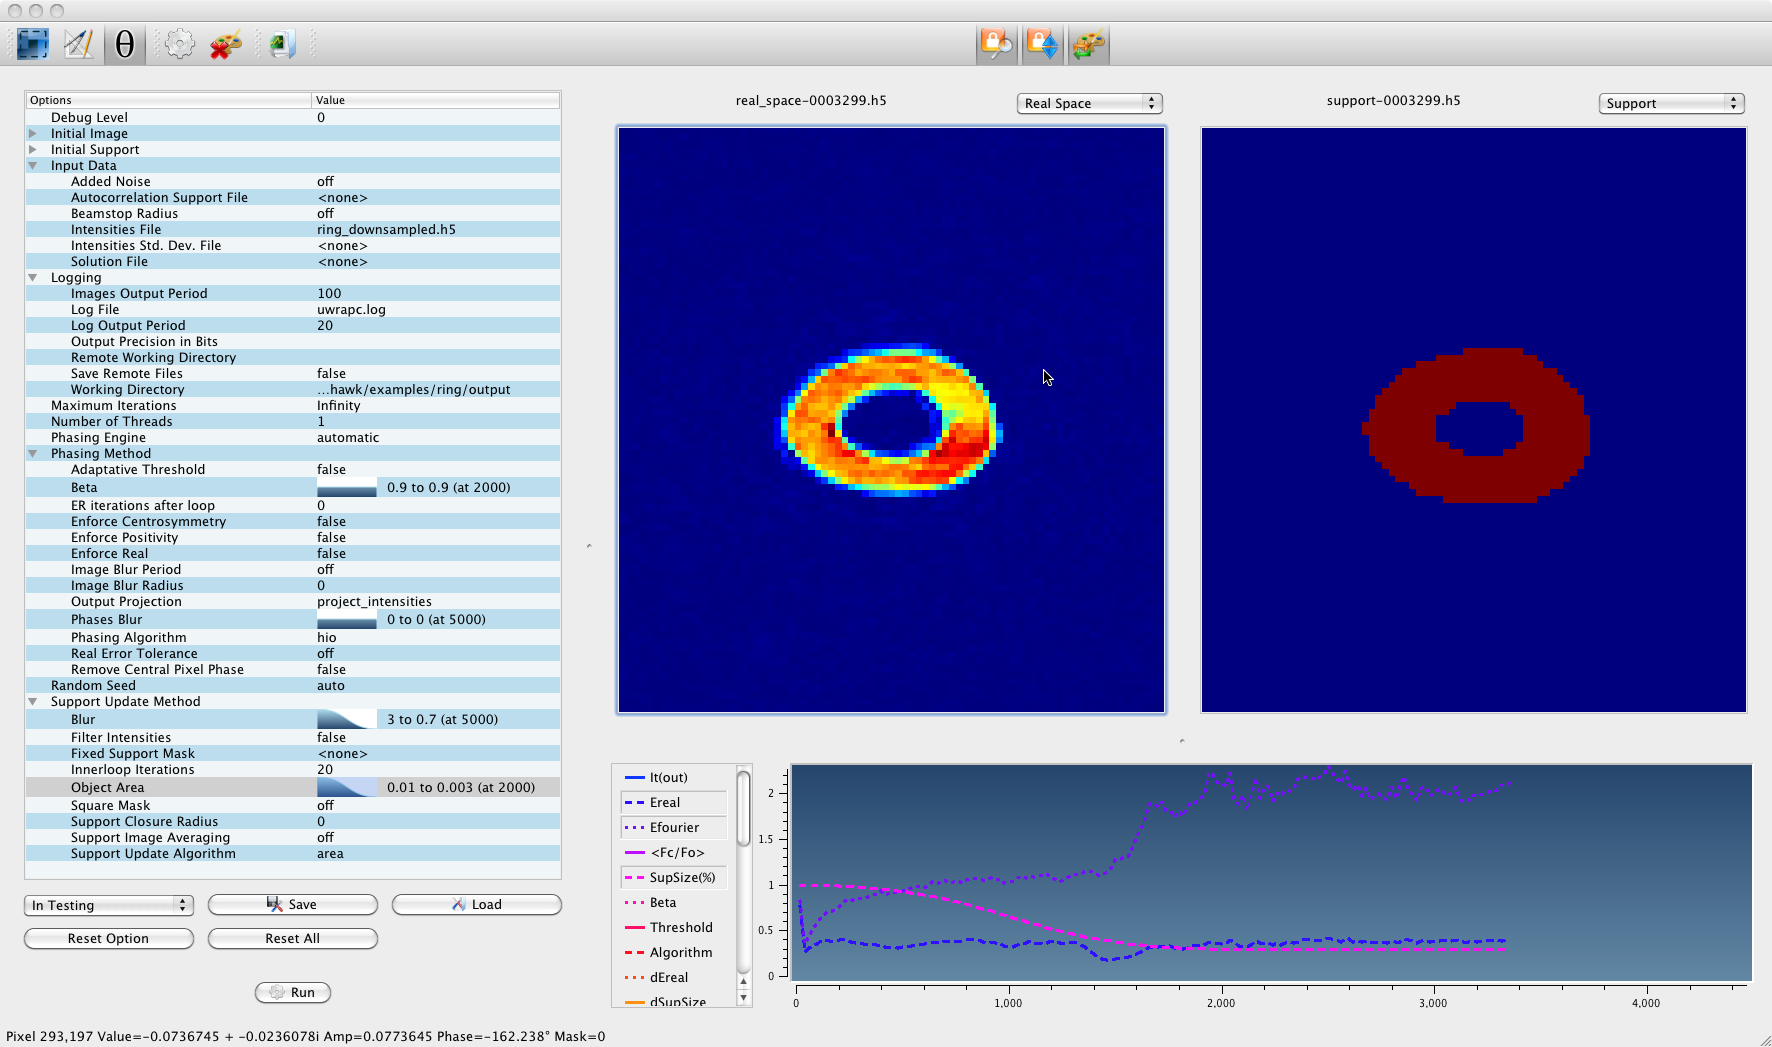
\includegraphics[width=1\textwidth]{reconstructed-ring.png}
\caption{Final result showing the reconstructed ring.}
\label{reconstructed-ring}
\end{figure}

If you did not succeed you can try to slightly adjust the parameters
until you get better results. Most of your time reconstructing images
will be spent doing just this.

Good luck in your future reconstructions!
%\bibliographystyle{acm}
%\bibliography{imaging}

\end{document}
 